\documentclass[oneside,reqno]{amsart}
\setlength{\textwidth}{\paperwidth}\addtolength{\textwidth}{-2in}\calclayout
\usepackage[utf8]{inputenc}
\usepackage{enumitem}
\usepackage{tikz}
\usepackage{minted}\newminted{python3}{frame=lines}
\usepackage{dsfont}
\usepackage{booktabs}

\DeclareMathOperator{\var}{var}
\DeclareMathOperator{\cov}{cov}
\DeclareMathOperator{\tr}{tr}
\DeclareMathOperator{\diag}{diag}
\DeclareMathOperator{\rank}{rank}
\newcommand{\eps}{\varepsilon}
\newcommand{\ups}{\upsilon}
\newcommand{\R}{\mathds R}
\newcommand{\Z}{\mathds Z}

\theoremstyle{definition}
\newtheorem{prob}{Problem}
\renewcommand*{\proofname}{Solution}
\setlist[enumerate]{label={(\roman*)}}

\title{ECON 706: Problem Set 8}
\author{Daniel Pfeffer}
%------------------------------------------------------------------------------
\begin{document}
\maketitle

\begin{prob}
Suppose that you have an AR(1) process of the form 
\begin{equation}\label{eq:ar1}
	y_t = \rho y_{t-1} + \eps_t,
	\qquad \eps_t \sim N(0,1).
\end{equation}
Now consider a two-state Markov process with $s_t \in \{s_1, s_2\}$ with transition matrix
\begin{equation}\label{eq:P}
	P = \begin{pmatrix}
		p_{11} & 1-p_{11} \\
		1- p_{22} & p_{22}
	\end{pmatrix}.
\end{equation}
Here, $p_{ij}$ is the probability of transitioning from state $s_1$ to state $s_2$. The Markov process has four parameters: $\theta = (p_{11}, p_{22}, s_1, s_2)$. We will try to approximate the AR(1) process $y_t$ in \eqref{eq:ar1} by the Markov process $s_t$ indexed by $\theta$.
\end{prob}

\begin{enumerate}[label=(\roman*)]
\item
Derive the eigenvalues associated with $P$ in \eqref{eq:P} as a function of $\theta$. 
\begin{proof}
The characteristic polynomial is
\begin{align*}
	\det(P - \lambda I) &= (p_{11} - \lambda )(p_{22} - \lambda) - (1-p_{11})(1-p_{22}) = 0 \\
	& = \lambda^2 - \lambda (p_{11} + p_{22}) + p_{11}p_{22} - 1 + p_{11} p_{22} - p_{11}p_{22} \\
	& = \lambda^2 - \lambda (p_{11} + p_{22}) - (1 - p_{11} - p_{22}),
\end{align*}
and has two eigenvalues given by
\begin{align*}
	\lambda &= \frac{p_{11} + p _{22}}{2} \pm \sqrt{\frac{(p_{11} + p _{22})^2}{4} +1 - \frac{2(p_{11} + p _{22})}{2}} \\
	&= \frac{p_{11} + p _{22}}{2} \pm \left(1 - \frac{p_{11} + p _{22}}{2} \right),
\end{align*}
with solutions $\lambda_1 = 1$ and $\lambda_2=  p_{11}+p_{22}-1$.
\end{proof}
\item
Derive the equilibrium distribution associated with $P$ as a function of $\theta$.
\begin{proof}
Let $\pi = (\pi_1, \pi_2)$ denote the invariant distribution of $P$, i.e., the (left) eigenvector corresponding to the eigenvalue $\lambda_1 = 1$. Then we know that $\pi$ must satisfy $\pi P = \pi$. i.e.,
\[
		(\pi_1,  \pi_1)
	 \begin{pmatrix}
		p_{11} & 1-p_{11} \\
		1- p_{22} & p_{22}
	\end{pmatrix}
	=(\pi_1,  \pi_1),
\]
which is an underdetermined system. Imposing a normalization restriction on $\pi$ (i.e., the probabilities sum to one) yields
\[
	\begin{cases}
		p_{11} \pi_1 + (1- p_{22}) \pi_2 = \pi_1 \\
		(1-p_{11}) \pi_1 + p_{22} \pi_2 = \pi_2
	\end{cases}
	\implies  
	\begin{cases}
		(1-p_{11}) \pi_1 =  (1- p_{22}) \pi_2 \\
		\pi_1 + \pi_2 = 1
	\end{cases},
\]
which has solution or equilibrium distribution given by
\[
	\pi = \left(\frac{1-p_{22}}{2-p_{11}  - p_{22}}, \frac{1-p_{11}}{2-p_{11} - p_{22}} \right).
\]     
\end{proof}
\item
For the $s_t$ process to approximate the $y_t$ process well, what properties would you like it to satisfy? Another way of asking the question is: think of a discrepancy measure between the processes $\{s_t\}_{t=-\infty}^\infty$ and $\{y_t\}_{t=-\infty}^\infty$.
\begin{proof}
We would like $s_t$ to have the same covariance structure as $y_t$, that is, we minimize 
\[
	\sum_{\tau\in \Z} \frac{|\gamma_y(\tau) - \gamma_s(\tau)|}{\gamma_y(0)}
\] 
with resect to $\gamma_s$. approximate the AR(1) process \eqref{eq:ar1} by requiring the $s_t$ process to have the same first and second order properties as the $y_t$ process. This provides a reasonable discrepancy measure between the two processes, since the autocovariance functions is a fundamental representation of the $y_t$ process. This method due to Tauchen (1986). 
\end{proof}
\item
Based on your notion of discrepancy, explain how you would choose $\theta$  approximate a continuous AR(1) process characterized by the parameters $\rho$, $\sigma^2$.
\begin{proof}
The Markov process admits a scalar AR(1) representation of the form 
\[
	s_t  = (1 - p_{11}) + (p_{11} + p_{22}-1) s_{t-1} + \eta_t,
\]
where the autoregressive coefficient is $p_{11} + p_{22}-1$, the second eigenvalue $\lambda_2$. We will approximate the continuous AR(1) processes \eqref{eq:ar1} as follows. Let us first set $s_2 =  -s_1$. We now derive two moment conditions; given $s_{t-1}=s_2$, the conditional mean and variance of $s_t$ satisfy 
\begin{align*}
	E(s_t \mid s_{t-1}=s_2) &= (1-p_{22}) s_2  + p_{22}s_2 = \rho s_2 \\
	\var(s_t \mid s_{t-1} = s_2) &= (1-p_{22}) (-s_2 -\rho s_2^2)^2 + p_{22}(s_2^2 - \rho s_2^2)^2 = 1.
\end{align*}
The first moment condition implies that 
\[
	p_{22} = p_{11} = \frac{1+\rho}{2},
\]
and the second moment condition, together which the previous implication, yields 
\[
	s_2 = -s_2 = \frac{\sigma}{\sqrt{1-\rho^2}}.
\]
This implies $\pi_1 = \pi_2 = 1/2$. To show that this method makes our discrepancy measure is zero, begin by inducting on $\tau$ to show that
\[
	P^\tau = \begin{pmatrix}
		\frac{1+\rho^\tau}{2} & \frac{1- \rho^\tau}{2} \\
		\frac{1-\rho^\tau}{2} & \frac{1+ \rho^\tau}{2}
	\end{pmatrix}.
\] 
The claim holds for the one-step ahead transition since
\[
	(1/2, 1/2)
	\begin{pmatrix}
		\frac{1+\rho}{2} & \frac{1- \rho}{2} \\
		\frac{1-\rho}{2} & \frac{1+ \rho}{2}
	\end{pmatrix}
	=\begin{pmatrix}
		\frac{1+\rho}{2} & \frac{1- \rho}{2} \\
		\frac{1-\rho}{2} & \frac{1+ \rho}{2}
	\end{pmatrix}.
\]
Assume the discrepancy measure is zero for $\tau$. Then for $\tau+1$,
\[
	(1/2, 1/2)
	\begin{pmatrix}
		\frac{1+\rho^\tau}{2} & \frac{1- \rho^\tau}{2} \\
		\frac{1-\rho^\tau}{2} & \frac{1+ \rho^\tau}{2}
	\end{pmatrix}
	=\begin{pmatrix}
		\frac{1+\rho^\tau}{2} & \frac{1- \rho^\tau}{2} \\
		\frac{1-\rho^\tau}{2} & \frac{1+ \rho^\tau}{2}
	\end{pmatrix}.
\]
Next, since by construction $E s_t = 0$, the autocovariance function of $s_t$ is 
\begin{align*}
	\gamma_s(\tau) &= E s_ts_{t+\tau} = E s_t E (s_{t+\tau} \mid s_t) \\
		&= \pi_1 s_1 E (s_{t+\tau} \mid s_t = s_1) +  (1-\pi_1) s_2 E (s_{t+\tau} \mid s_t = s_2) \\
		&= \frac{1}{2} s_1 \left(\frac{1+\rho^2}{2} s_1^2 + \frac{1-\rho^2}{2} s_2\right) + \frac{1}{2} s_2 \left(\frac{1+\rho^2}{2} s_1^2 + \frac{1-\rho^2}{2} s_2 \right) \\
		&= \frac{1}{2} \frac{1+\rho^2}{2} s_1^2 + \frac{1-\rho^2}{2} s_1s_2 + \frac{1}{2} \frac{1+\rho^2}{2} s_2 \\
		&= \frac{\sigma^2}{1-\rho^2}\rho^\tau = \gamma_y(\tau),
\end{align*}
the desired result.
\end{proof}
\item
Choose values for $\rho$, $\sigma^2$, compute your proposed $\theta$, then simulate the two processes and compare the sample autocovariance functions.
\begin{proof} 
We set $\rho = 0.5$ and $\sigma^2=1$. The following code generates a two state Markov chain approximation for this AR(1) process. Then the ``true'' AR(1) process is simulated. Figure \ref{markov-ar1-acf-fig} shows the resulting sample autocorrelation functions. Visual inspection suggests that, even with relatively high persistence, we can obtain a reasonable discretized approximation taking values $s_t \in \{s_1, s_2\}$ to the continuous-valued AR(1) process.
\begin{python3code}
import numpy as np
import matplotlib.pyplot as plt
from scipy.stats import norm
from statsmodels.tsa.stattools import acf

# Simulation parameters 
sigma = 1
rho = 0.5

# Tauchen chain
s = sigma / np.sqrt(1-rho**2)
S = [s, -s]
p = (1 + rho) / 2
P = [[p, 1-p], [1-p, p]]

# Simulate the AR(1) process and Tauchen chain
np.random.seed(42)
T = 100
y_path, s_path = [s], [s]
mu = norm.rvs(loc=0, scale=sigma, size=T)
for t in range(T):
    y_path.append(rho*y_path[t] + mu[t])
    
    tr_pr = (s_path[t] == s)*P[0] + (s_path[t] == -s)*P[1]
    
    # Inverse cdf method with corresponding sample
    cdf_val = 1 - norm.cdf(mu[t])
    s_path.append((cdf_val < tr_pr[0])*s + (cdf_val > tr_pr[0])*(-s))

# Acfs
tauchen_acf = acf(s_path, fft=False)
ar1_acf = acf(y_path, fft=False)

# Plot sample paths and acfs
plt.figure(figsize=(10,4))

ax1 = plt.subplot(121)
plt.plot(y_path, label='AR(1)')
plt.plot(s_path,'o', label='Chain')
plt.legend()
plt.title('Sample Path')

ax2 = plt.subplot(122)
plt.plot(ar1_acf)
plt.plot(tauchen_acf)
plt.title('Autocorrelation')

plt.show()
\end{python3code}

\begin{figure}
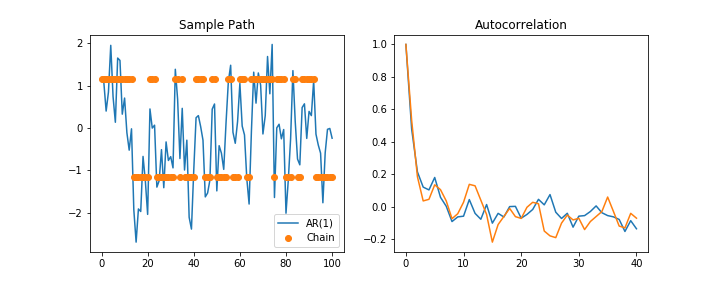
\includegraphics[width=\textwidth]{q1-sim}
\caption{Sample autocorrelation functions for simulated sample paths $\{y_t\}_{t=0}^{100}$ and $\{s_t\}_{t=0}^{100}$.}
\label{markov-ar1-acf-fig}
\end{figure}

\end{proof}
\end{enumerate}


\begin{prob}
Consider the vector error correction model
\begin{equation}\label{eq:vecm}
	\Delta y_t = \Pi_0 + \alpha \beta' y_{t-1} + \sum_{j=1}^{p-1} \Pi_j \Delta y_{t-j} + \eps_t, 
	\qquad \eps_t \sim N(0, \Sigma).
\end{equation}
\end{prob}

\begin{enumerate}[label=(\roman*)]
\item
Rewrite the system as VAR in levels:
\begin{equation}\label{eq:levels}
	y_t = \Phi_0 + \sum_{j=1}^p \Phi_j y_{t-j} + \eps_t.
\end{equation}
What is the relationship between the $\Phi$ matrices in \eqref{eq:levels} and the $\Pi$ matrices in \eqref{eq:vecm}?
\begin{proof}
We have
\[
	y_t - y_{t-1} = \Pi_0 + \alpha \beta' y_{t-1} + \Pi_1 (y_{t-1}  - y_{t-2}) +  \cdots  + \Pi_{p-1} (y_{t-p+1}  - y_{t-p}) + \eps_t,
\]
which, after rearranging, becomes a VAR($p$) in levels of the form
\begin{align*}
	y_t  &= \Pi_0 +  (\alpha \beta' + \Pi_1 + I)y_{t-1}  +(\Pi_2 - \Pi_1) y_{t-2} + \cdots + (\Pi_{p-1} - \Pi_{p-2})  y_{t-p} - \Pi_{p-1}y_{t-p} + \eps_t \\
	&= \Phi_0 +  \Phi_1 y_{t-1}  + \Phi_2 y_{t-2} + \cdots + \Phi_p y_{t-p} + \eps_t
\end{align*}
where 
\begin{align*}
	\Phi_0 &= \Pi_0 \\
	\Phi_1 &=  \alpha \beta' + \Pi_1 + I \\
	\Phi_j &= \Pi_j - \Pi_{j-1} \qquad \text{for } j = 2,\dotsc, p-1 \\
	\Phi_p &= - \Pi_{p-1},
\end{align*} 
.
\end{proof}
\item
Get quarterly data on nominal GDP and nominal investment from the
FRED database (there are different types of aggregate investment series,
just pick one of them and report which one you chose.) Plot log GDP
and investment, as well as the log investment-to-GDP ratio. Comment
on the trends in these three series over different periods of time.
\begin{proof}
Figure \eqref{macro-series} shows log GDP and log gross private domestic investment (left), as well as  log investment-to-GDP ratio (right) for 1984:Q1 through 2019:Q4. Both GDP and investment exhibit a linear trend in logs, and hence are nonstationary. The difference in values (i.e., ratio in levels), however, remain relatively constant. Moreover, the somewhat random fluctuations in the log investment-to-GDP ratio have characteristics of white noise, providing evidence of a common stochastic trend component shared by these series'. It should be noted that log investment is more volatile than log GDP, as can be seen around 1992 and 2004 through 2008. This observation is also seen in the log investment-to-GDP ratio at the corresponding time periods. This observed non-constant variance suggests that the log investment-to-GDP ratio may not be white noise. Code is used to generate these plots is presented below.

\begin{figure}
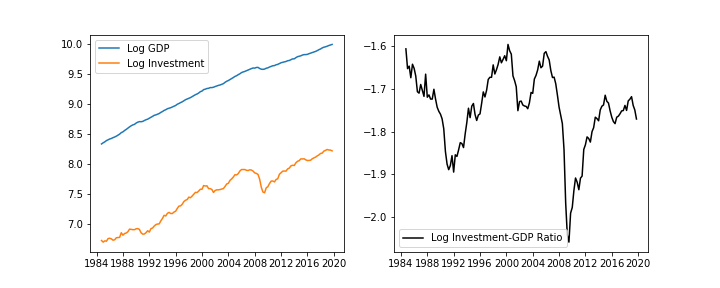
\includegraphics[width=\textwidth]{macro-series}
\caption{All data are nominal.}
\label{macro-series}
\end{figure}

\begin{python3code}
import pandas_datareader.data as web
import datetime

# 1984:Q1 to 2015:Q4
start = datetime.datetime(1984, 10, 1)
end = datetime.datetime(2019, 12, 31)

# Quarterly U.S. real GDP from the FRED
ts = web.DataReader(['GPDI', 'GDP'], 'fred', start, end)

y = pd.DataFrame({'log_inv': np.log(ts['GPDI']),
                  'log_gdp':np.log(ts['GDP'])})
                  
fig, (ax1, ax2) = plt.subplots(1, 2, figsize=(10,4))

ax1.plot(y['log_gdp'], label='Log GDP')
ax1.plot(y['log_inv'], label='Log Investment')
ax1.legend()

ax2.plot(y['log_inv'] - y['log_gdp'], 'k', label='Log Investment-GDP Ratio')
ax2.legend()

plt.show()
\end{python3code}
\end{proof}

\item
Define $y_t = (\log \text{Inv}_t, \log \text{GDP}_t)'$. Set $p=4$ and assume that the cointegration vector is $\beta=(1,-1)'$. Estimate \eqref{eq:vecm} and \eqref{eq:levels}, by OLS (over the same time period), setting $p=4$. 

\begin{proof}
Under these assumptions, the VECM becomes 
\[
	\Delta y_{it} = \Pi_{i0} + \alpha_i (y_{1,t-1} - y_{2,t-1}) + \sum_{j=1}^3 ( (\Pi_j)_{i1} \Delta y_{1,t-j} + (\Pi_j)_{i2} \Delta y_{2,t-j} ) + \eps_{it},
	\qquad i=1,2.
\]
The following code estimates the VECM and VAR models from 1984:Q1 through 2019:Q4. 
\begin{python3code}
from statsmodels.tsa.api import VAR, VECM

y = ts[['log_inv', 'log_gdp']]
vecm_mod = VECM(y, k_ar_diff=3, deterministic='co', coint_rank=1, freq='QS')
vecm_res = vecm_mod.fit()

var_mod = VAR(y, freq='QS')
var_res = var_mod.fit(4)
\end{python3code}

The estimated VECM coefficients $\widehat \Pi$ are $\widehat\Pi_0 = (-0.286, 0.025)'$,
\footnote{All coefficient matries throughout are of the form 
\[
	\bordermatrix{~ & \text{Investment} & \text{GDP} \cr
                 \text{Investment} & \star & \star \cr
                  \text{GDP} & \star & \star \cr}.
\]}
\begin{alignat*}{2}
	\alpha\beta' &= \begin{pmatrix}
		-0.080 & 0.093 \\
		 0.006 & -0.007
	\end{pmatrix}  \qquad &&
	\widehat\Pi_1 = \begin{pmatrix}
		-0.113 & 2.684 \\
		-0.002 & 0.319
	\end{pmatrix} \\
	\widehat\Pi_2 &=\begin{pmatrix}
		0.060 & 1.094 \\
		0.010 & 0.151
	\end{pmatrix} \qquad &&
	\widehat\Pi_3 = \begin{pmatrix}
		0.044 & -0.727 \\
		-0.007 & 0.005
	\end{pmatrix}.
\end{alignat*}
The estimates $\widehat \Phi$ are $\widehat \Phi_0 = (-0.260,0.031)'$,
\begin{alignat*}{2}
	\widehat \Phi_1 &= \begin{pmatrix}
		0.807 & 2.669 \\
		 0.004 & 1.285
	\end{pmatrix} \qquad &&
	\widehat \Phi_2= \begin{pmatrix}
		0.177 & -1.562 \\
		0.012 & -0.160
		\end{pmatrix} \\
	\widehat \Phi_3 &= \begin{pmatrix}
		-0.009 & -1.814 \\
		-0.016 & -0.145 
	\end{pmatrix} \qquad&&
	\widehat \Phi_4  = \begin{pmatrix}
		-0.080 & 0.818 \\
		-0.002 & 0.018
	\end{pmatrix}.
\end{alignat*}
\end{proof}

\item
Convert the estimates $\widehat \Pi$ into estimates $\widetilde \Phi$ obtained using the relationship derived in part (i). Compare the $\widetilde \Phi$ estimates obtained indirectly by estimating the VECM, to the $\widehat\Phi$ by estimating (4) directly. We did not develop enough econometric theory to conduct a formal test of whether the underlying parameters are identical and the VECM restrictions are satisfied, but please comment on the similarity of the estimates.

\begin{proof}
We now compute VAR coefficeints implied by the above estimates.
\begin{python3code}
# VAR implied by VECM 
vecm_res.var_rep
\end{python3code}

The implied estimates $\widetilde \Phi$ are
\begin{alignat*}{2}
	\widetilde \Phi_1 &= \begin{pmatrix}
		0.807 & 2.777 \\ 
		0.004 & 1.312
	\end{pmatrix} \qquad &&
	\widetilde \Phi_2= \begin{pmatrix}
		 0.172 & -1.590 \\ 
		0.012 & -0.167
	\end{pmatrix} \\
	\widetilde \Phi_3 &= \begin{pmatrix}
		 -0.016 & -1.821 \\ 
		-0.017 & -0.147
	\end{pmatrix} \qquad&&
	\widetilde \Phi_4  = \begin{pmatrix}
		-0.044 &  0.727  \\ 
		0.007 & -0.005 
	\end{pmatrix}.
\end{alignat*}
The VAR estimates implied by the VECM model $\widetilde \Phi$ differ only slightly from the $\widehat\Phi$ estimates. We get this result since $\Phi_1$ as define in (i) captures the cointegrating relation and $\Phi_2, \Phi_3$, and $\Phi_4$ capture the proposed white noise in the cointegrating residuals. \end{proof}

\item
Starting from the last $p$ observations in your sample iterate (3) and
(4) forward conditional on their respective OLS parameter estimates.
Compare the implied paths of $\log \text{Inv}_t$ and $\log \text{GDP}_t$ over the next ten years (forty quarters) by generating plots that show the actual time series until period T and overlay the model-implied paths for $t=T+1$
to $t = T + 40$. Note that the VECM gives you a path for $\Delta y_t$ that you have to convert into a path for $y_t$ (alternatively, you could work with the
result derived in (i)).

\begin{proof}
Forecasts for nominal GDP and investment are generated below. Figure \ref{q2-nominal} shows that both models forecast (dashed lines) an upward trend, with the VECM making a slightly more aggressive forecast. The following code forecasts the VECM model and VAR model. 

\begin{python3code}
# Forecasts
vecm_forecast = np.vstack([y.values, vecm_res.predict(40)])
var_forecast = np.vstack([y.values, var_res.forecast(y.values, steps=40)])

x = [i for i in range(len(vecm_forecast))]

plt.figure(figsize=(10,4))

# Historical Data
plt.plot(x[:141], var_forecast[:141,1], label='GDP')
plt.plot(x[:141], vecm_forecast[:141,0], label='Inv')

# GDP Forecast
plt.plot(x[141:], var_forecast[141:,1], 'g--')
plt.plot(x[141:], vecm_forecast[141:,1], 'r--')

# Investment Forecast
plt.plot(x[141:], var_forecast[141:,0], 'g--', label='VAR')
plt.plot(x[141:], vecm_forecast[141:,0], 'r--', label='VECM')

plt.legend()
plt.title('Nominal GDP and Investment')

plt.show()
\end{python3code}

\begin{figure}
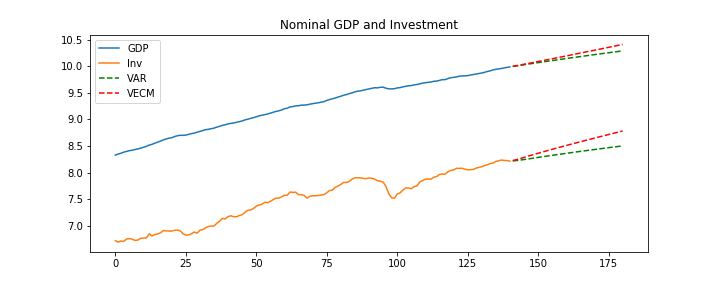
\includegraphics[width=\textwidth]{q2-nominal}
\caption{VECM and VAR 10 year forecasts for nominal investment and GDP.}
\label{q2-nominal}
\end{figure}
\end{proof}

\item
Repeat the computations for measures of real investment and real GDP.
Why is the ratio of nominal investment and nominal GDP different from the ratio of real investment and real GDP?

\begin{proof}
Query real investment and GDP data from 1984:Q1 to 2019:Q4 and plot the observed series.
\begin{python3code}
# Quarterly U.S. real GDP and real investment from the FRED
ts = web.DataReader(['GPDIC1', 'GDPC1'], 'fred', start, end)
    
x = pd.DataFrame({'log_inv': np.log(ts['GPDIC1']),
                  'log_gdp':np.log(ts['GDPC1'])})

# Plot data
fig, (ax1, ax2) = plt.subplots(1, 2, figsize=(10,4))

ax1.plot(x['log_gdp'], label='Log GDP')
ax1.plot(x['log_inv'], label='Log Investment')
ax1.legend()

ax2.plot(x['log_inv'] - x['log_gdp'], 'k', label='Log Investment-GDP Ratio')
ax2.legend()

plt.show()
\end{python3code}

Figure \ref{real-macro-series} shows log real GDP and log real private domestic investment, as well as the log investment-GDP ratio. Evidently, the aforementioned volatility observed in Figure \ref{macro-series}, is less apparent when the series are viewed in real terms. As a result, the log investment-GDP ratio looks less like a white noise process as previously suggested. A possible explanation for this observation could be that inflation is, in some sense, is acting as measurement error in the nominal series, resulting in increased noise, and hence making the series look more like a totally random process. Albeit, this speculation is doubtful, especially when viewed in light of the ``Slutzky  effect'' (1937). The following code repeats the above computations for real GDP and real investment. 

\begin{figure}
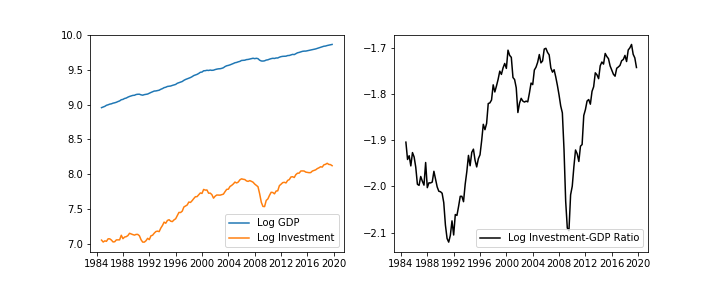
\includegraphics[width=\textwidth]{real-macro-series}
\caption{Data are in real terms.}
\label{real-macro-series}
\end{figure}

Fit VECM and VAR model on real investment and GDP.
\begin{python3code}
# Real VECM model
rvecm_mod = VECM(x, k_ar_diff=3, deterministic='co',
                coint_rank=1, freq='QS')
rvecm_res = rvecm_mod.fit()

# Real VAR model
rvar_mod = VAR(x, freq='QS')
rvar_res = var_mod.fit(4)
\end{python3code}

The estimated VECM coefficients $\widehat \Pi$ are $\widehat\Pi_0 = (-0.286, 0.025)'$,
\begin{alignat*}{2}
	\alpha\beta' &= \begin{pmatrix}
		  -0.133 & 0.204  \\
		  0.003 & -0.005
	\end{pmatrix}  \qquad &&
	\widehat\Pi_1 = \begin{pmatrix}
		-0.113 & 2.684 \\
		 -0.002 & -0.319
	\end{pmatrix} \\
	\widehat\Pi_2 &=\begin{pmatrix}
		0.060 &  1.094 \\
		 -0.010 & 0.151
	\end{pmatrix} \qquad &&
	\widehat\Pi_3 = \begin{pmatrix}
		0.044 &  -0.727 \\
		 -0.007 & 0.005
	\end{pmatrix}.
\end{alignat*}
The estimates $\widehat \Phi$ are $\widehat \Phi_0 = (-0.2596,0.0320)'$,
\begin{alignat*}{2}
	\widehat \Phi_1 &= \begin{pmatrix}
		 0.870 &  2.669 \\
		 0.004 & 1.285
	\end{pmatrix} \qquad &&
	\widehat \Phi_2= \begin{pmatrix}
		0.177 & -0.177 \\
		 0.013 & -0.160
		\end{pmatrix} \\
	\widehat \Phi_3 &= \begin{pmatrix}
		 -0.009 & -1.814 \\
		 0.016 & -0.145 
	\end{pmatrix} \qquad&&
	\widehat \Phi_4  = \begin{pmatrix}
		-0.080 &  0.818 \\
		 -0.002 & 0.018
	\end{pmatrix}.
\end{alignat*}

Compute the VAR coefficients implied by the VECM.
\begin{python3code}
# VAR representation implied by VECM
rvecm_res.var_rep
\end{python3code}

The VAR coefficients implied by the VECM model are 
\begin{alignat*}{2}
	\widetilde \Phi_1 &= \begin{pmatrix}
		 0.069 &  3.172 \\
		0.001 &  1.269
	\end{pmatrix} \qquad &&
	\widetilde \Phi_2= \begin{pmatrix}
		0.010 & -0.860 \\ 
		0.004 & -0.005
	\end{pmatrix} \\
	\widetilde \Phi_3 &= \begin{pmatrix}
		 0.010 & -2.282 \\ 
		-0.001 & -0.023
	\end{pmatrix} \qquad&&
	\widetilde \Phi_4  = \begin{pmatrix}
		-0.003 & 0.018 \\
        		0.009 &  0.005
	\end{pmatrix}.
\end{alignat*}
Comparing $\widetilde \Phi$ to the estimated VAR coefficients, we can see that the magnitude of differences of these coefficient matrices is less than the previous differences observed in (iii).
\par
Generate 10 year ahead forecast. 
\begin{python3code}
# VECM and VAR forecasts
rvecm_forecast = np.vstack([x.values, rvecm_res.predict(40)])
rvar_forecast = np.vstack([x.values, rvar_res.forecast(x.values, steps=40)])

# Plot results
rx = [i for i in range(len(rvecm_forecast))]

plt.figure(figsize=(10,4))

# Historical data
plt.plot(rx[:141], rvar_forecast[:141,1],  label='GDP')
plt.plot(rx[:141], rvecm_forecast[:141,0], label='Inv')

# Investment forecasts
plt.plot(rx[141:], rvar_forecast[141:,0], 'g--', label='VAR')
plt.plot(rx[141:], rvecm_forecast[141:,0], 'r--', label='VECM')

# GDP forecasts
plt.plot(rx[141:], rvar_forecast[141:,1], 'r--')
plt.plot(rx[141:], rvecm_forecast[141:,1], 'g--')

plt.legend()
plt.title('Real GDP and Investment')

plt.show()
\end{python3code}

Forecasts for real GDP and investment are given in Figure \ref{q2-real} and both both lower than forecasts for their nominal counterparts. The VECM forecast shows declining growth while the VAR forecasts show constant growth. This again may be related the the earlier speculation that inflation is biasing our nominal estimates.

\begin{figure}
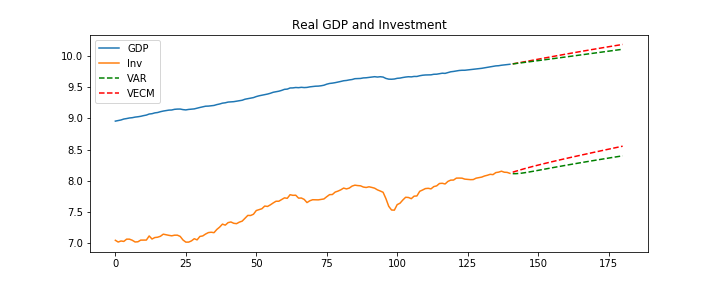
\includegraphics[width=\textwidth]{q2-real}
\caption{VECM and VAR 10 year forecasts for real investment and GDP.}
\label{q2-real}
\end{figure}

\end{proof}
\end{enumerate}

\end{document}



